\section{Scattering in QED II}
Recall the LSZ formula we found for $e^-e^-\to e^-e^-$
\begin{equation}
    i\mathcal{M}(p_1p_2\to p_3p_4) = i^4[\bar{u}_4(\slashed{p}_4 + m)]_\delta [\bar{u}_3(\slashed{p}_3 + m)]_\gamma \avg{\mathcal{T}\psi_\delta(p_4)\psi_\gamma(p_3)\bar{\psi}_\beta(p_2)\bar{\psi}_\alpha(p_1)}_C[(\slashed{p}_2 + m)u_2]_\beta[(\slashed{p}_1 + m)u_1]_\alpha
\end{equation}
One can similarly show that for $e^+e^+ \to e^+e^+$ (you will show this on the pset - though we can guess the solution. $\psi \sim b + d^\dag$, so):
\begin{equation}
    i\mathcal{M}(p_1p_2\to p_3p_4) = i^4[(-\slashed{p}_4 + m)v_4]_\delta [(-\slashed{p}_3 + m)v_3]_\gamma \avg{\mathcal{T}\bar{\psi}_\delta(p_4)\bar{\psi}_\gamma(p_3)\psi_\beta(p_2)\psi_\alpha(p_1)}_C[(\slashed{p}_2 + m)u_2]_\beta[(\slashed{p}_1 + m)u_1]_\alpha
\end{equation}

\subsection{$e^+e^-\to\mu^-\mu^+$ scattering}

The first scattering observable we will study is $e^+e^- \to \mu^-\mu^+$. The muon $\mu^-$ is also a Dirac fermion with charge $1$, so it couples to photons in a very similar way to electrons. However it is heavier, with $m_e \sim 0.5\si{MeV}$ and $m_\mu \sim 100\si{MeV}$. We will also look at electron-positron to electron-positron scattering, but this turns out to be easier since electrons and muons are distinguishable.

\begin{center}
    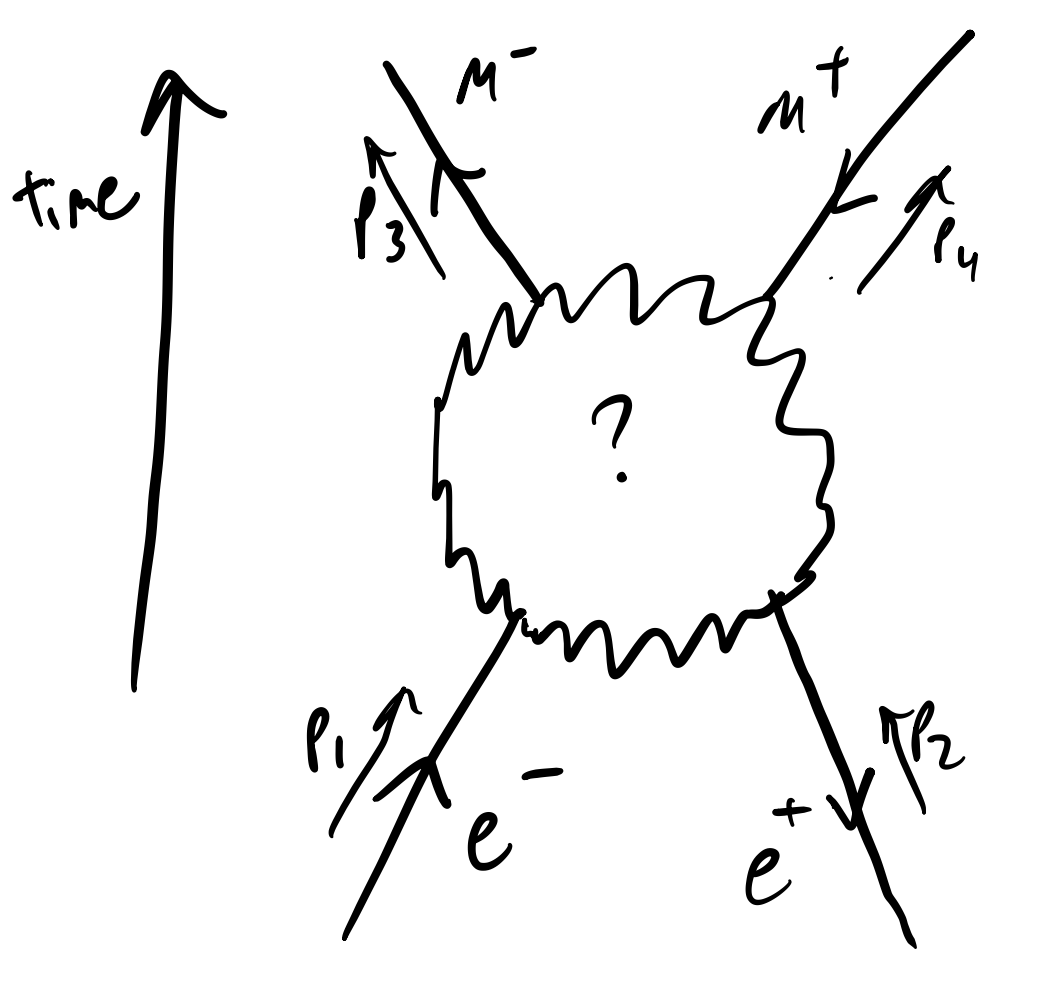
\includegraphics[scale=0.35]{Lectures/Images/lec13-mumuee.png}
\end{center}

The action of our system is:
\begin{equation}
    S = \int \bar{\psi}_e(i\slashed{D} - m_e)\psi_e + \bar{\psi}_\mu(i\slashed{D} - m_\mu)\psi_\mu - \frac{1}{4}F^2
\end{equation}
with:
\begin{equation}
    D_\mu \psi \p_\mu \psi + i e A_\mu \psi
\end{equation}
The LSZ formula tells us how to relate $\mathcal{M}$ to a connected 4-point function:
\begin{equation}
    i\mathcal{M} = i^4[(-\slashed{p}_4 + m)v_4]_\delta[\bar{u}_3(\slashed{p}_3 + m_\mu)]_\gamma\avg{\mathcal{T}\bar{\psi}^\mu_\delta(p_4)\psi^\mu_\gamma(p_3)\psi^e_\beta(p_2)\bar{\psi}^e_\alpha(p_1)}_c[\bar{v}_2(-\slashed{p}_2 + m)]_\beta[(\slashed{p}_1 + m)u_1]_\alpha
\end{equation}
Now, we calculate the correlation function using our knowledge of QED. The electrons and muons are connected via the photon field, which they are both coupled to. We will use the vertex:
\begin{equation}
    S_{\text{int}} = -e\int A_\nu(\bar{\psi}_e\gamma^\nu \psi_e + \bar{\psi}_\mu \gamma^\mu \psi_\mu)
\end{equation}
We will go to second order (intuitively - we need two powers in order to connect the $\psi_e$ and $\psi_\mu$ fields), and study the cross-terms:
\begin{equation}
    \frac{i^2}{2}S_{\text{int}}^2 = -\frac{e^2}{2}\int A \cdot (j_e + j_\mu)\int A\cdot (j_e + j_\mu) \supset -e^2\int A\cdot j_e\int A\cdot j_\mu
\end{equation}
We can drop the $(Aj_e)^2, (Aj_\mu)^2$ terms as they do not contribute to our observable of interest.

\begin{center}
    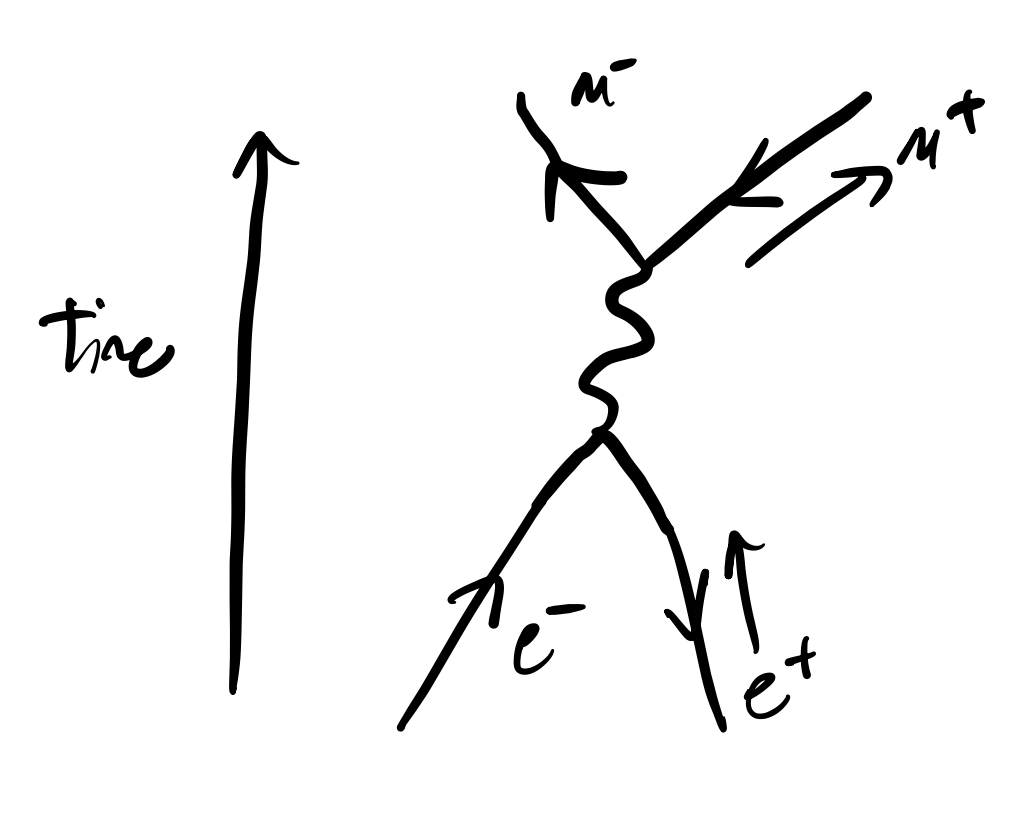
\includegraphics[scale=0.35]{Lectures/Images/lec13-mumueeschannel.png}
\end{center}

The leading contribution is thus:
\begin{equation}
    \avg{\bar{\psi}^\mu_\delta \psi^\mu_\gamma \psi^e_\beta \bar{\psi}^e_\alpha} = -e^2\avg{(\int A_\rho \bar{\psi}_\mu \gamma^\rho \psi_\mu)\bar{\psi}^\mu_\delta(p_4)\psi_\gamma^\mu(p_3)\psi_\beta^e(p_2)\bar{\psi}^e_\alpha(p_1)(\int A_\lambda \bar{\psi}^e \gamma^\lambda \psi^e)}_{\text{free}}
\end{equation}
and now we evaluate this via Wick contractions in the free theory; electrons must contract with electrons and muons must contract with muons. We contract $\psi^e$ with $\bar{\psi}_\alpha^e(p_1)$  (two exchanges so no minus) and $\psi^e_\beta(p_2)$ with $\bar{\psi}^e$, which yields:
\begin{equation}
    [G(-p_2)\gamma^\lambda G(p_1)]_{\beta\alpha}
\end{equation}
Doing the same story on the left with the muons (note there is now a minus sign to fermion exchanges), we get:
\begin{equation}
    -[G(-p_3)\gamma^\rho G(p_4)]_{\gamma\delta}
\end{equation}
Finally we contract the photons, and so at the end of the day we end up with (note that this was the unique possible choice of contractions):
\begin{equation}
    \avg{\bar{\psi}^\mu_\delta \psi^\mu_\gamma \psi^e_\beta \bar{\psi}^e_\alpha} = +e^2[G(-p_3)\gamma^\rho G(p_4)]_{\gamma\delta}G_{\rho\lambda}(p_1 + p_2)[G(-p_2)\gamma^\lambda G(p_1)]_{\beta\alpha}
\end{equation}
This is the expression for the 4-point function. Dotting it with the $(\slashed{p} + m)$ factors will simplify things because the Green's function is precisely the inverse!
\begin{equation}\label{eq:eemumu}
    \begin{split}
        i\mathcal{M} &= e^2(\bar{u}_3\gamma^\rho v_4)G_{\rho\lambda}(p_1 + p_2)(\bar{v}_2\gamma^\lambda u_1)
        \\ &= e^2(\bar{u}_3\gamma^\rho v_4)\frac{-i}{(p_1 + p_2)^2}(\eta_{\rho\lambda} + (\xi - 1)\frac{(p_1 + p_2)_{\rho}(p_1 + p_2)_\lambda}{(p_1 + p_2)^2})(\bar{v}_2\gamma^\lambda u_1)
        \\ &= \frac{ie^2}{s}(\bar{u}_3\gamma^\rho v_4)(\bar{v}_2\gamma_\rho u_1)
    \end{split}
\end{equation}
where $u_i = u_{s_i}(p_i)$, and in the third equality we use the fact that $\bar{v}_2(\slashed{p}_1 + \slashed{p}_2)u_1 = \bar{v}_2(-m + m)u_1 = 0$ to kill the $\xi$-dependent term. In the last equality we have recalled the definition of the Mandelstam variable $(p_1 + p_2)^2 = -s$.

\subsection{Comparing to the scalar, $e^-e^+ \to e^-e^+$ scattering}

Compare this to the scattering we found for the scalar:

\begin{center}
    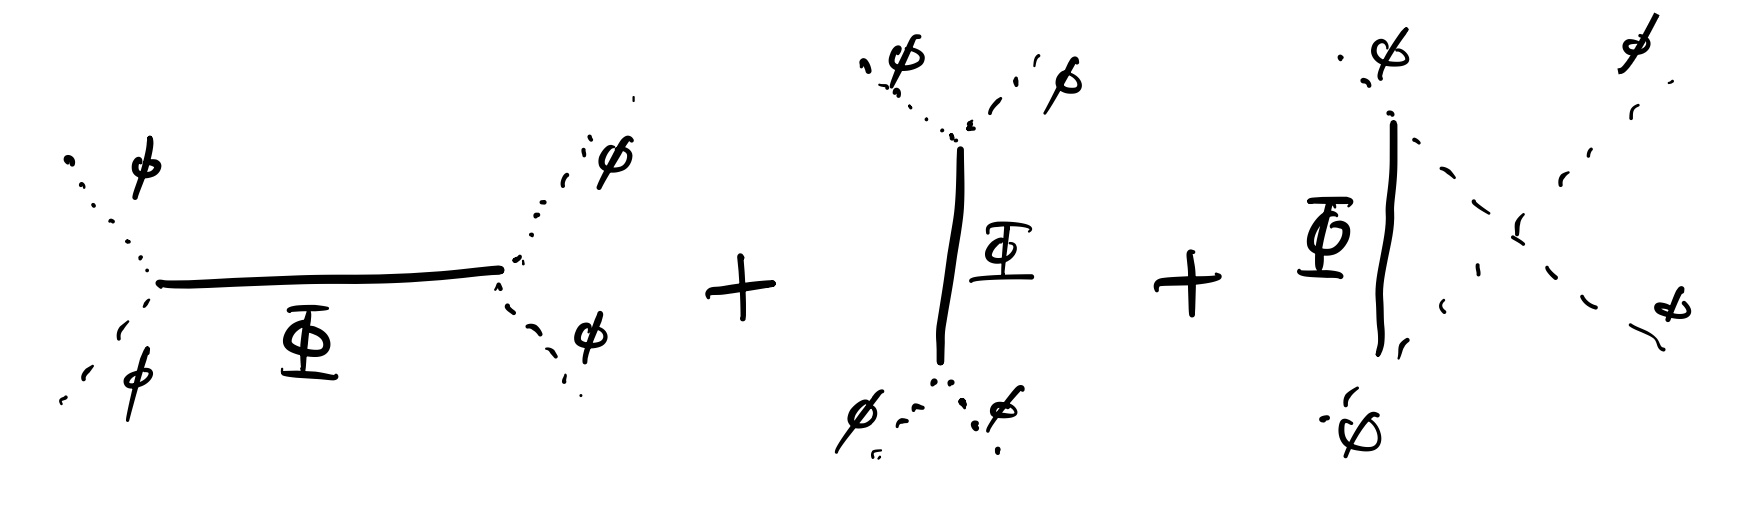
\includegraphics[scale=0.35]{Lectures/Images/lec13-scalarscatter.png}
\end{center}

where:
\begin{equation}
    \mathcal{M} \sim g^2\left(\frac{1}{s + M^2} + \frac{1}{t + M^2} + \frac{1}{u + M^2}\right)
\end{equation}
we note that with our QED scattering, the only contribution is from the $s$-channel, and since the photon is massless we do not have $M^2$ terms as we did for the massive ($\Phi$)-scalar mediated scattering. The third difference is that we have the $u/v$s which depend on the external spin and momenta.

\begin{center}
    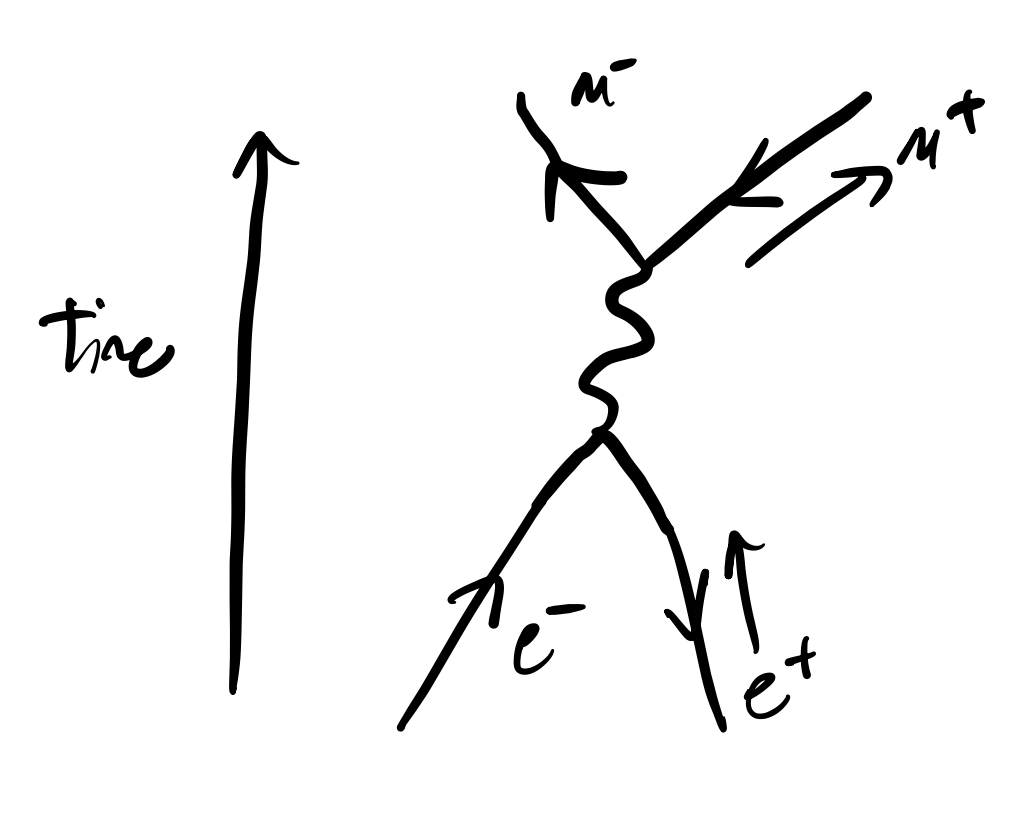
\includegraphics[scale=0.35]{Lectures/Images/lec13-mumueeschannel.png}
\end{center}

What about $e^-e^+ \to e^-e^+$ scattering? The same diagram is allowed, but there is another allowed diagram now coming from the fact that the we have two electron vertices (we get a $t$-channel  $t = -(p_1 - p_3)^2$ in addition to the $s$ channel $s = -(p_1 + p_2)^2$). This comes out of the Wick contractions, but pictorially we imagine that this second diagram corresponds to the electron staying as an electron, but radiating a photon which hits an incoming positron (as opposed to the $s$-channel diagram, which corresponds to an electron/positron pair ``becoming'' a muon/antimuon pair)

\begin{center}
    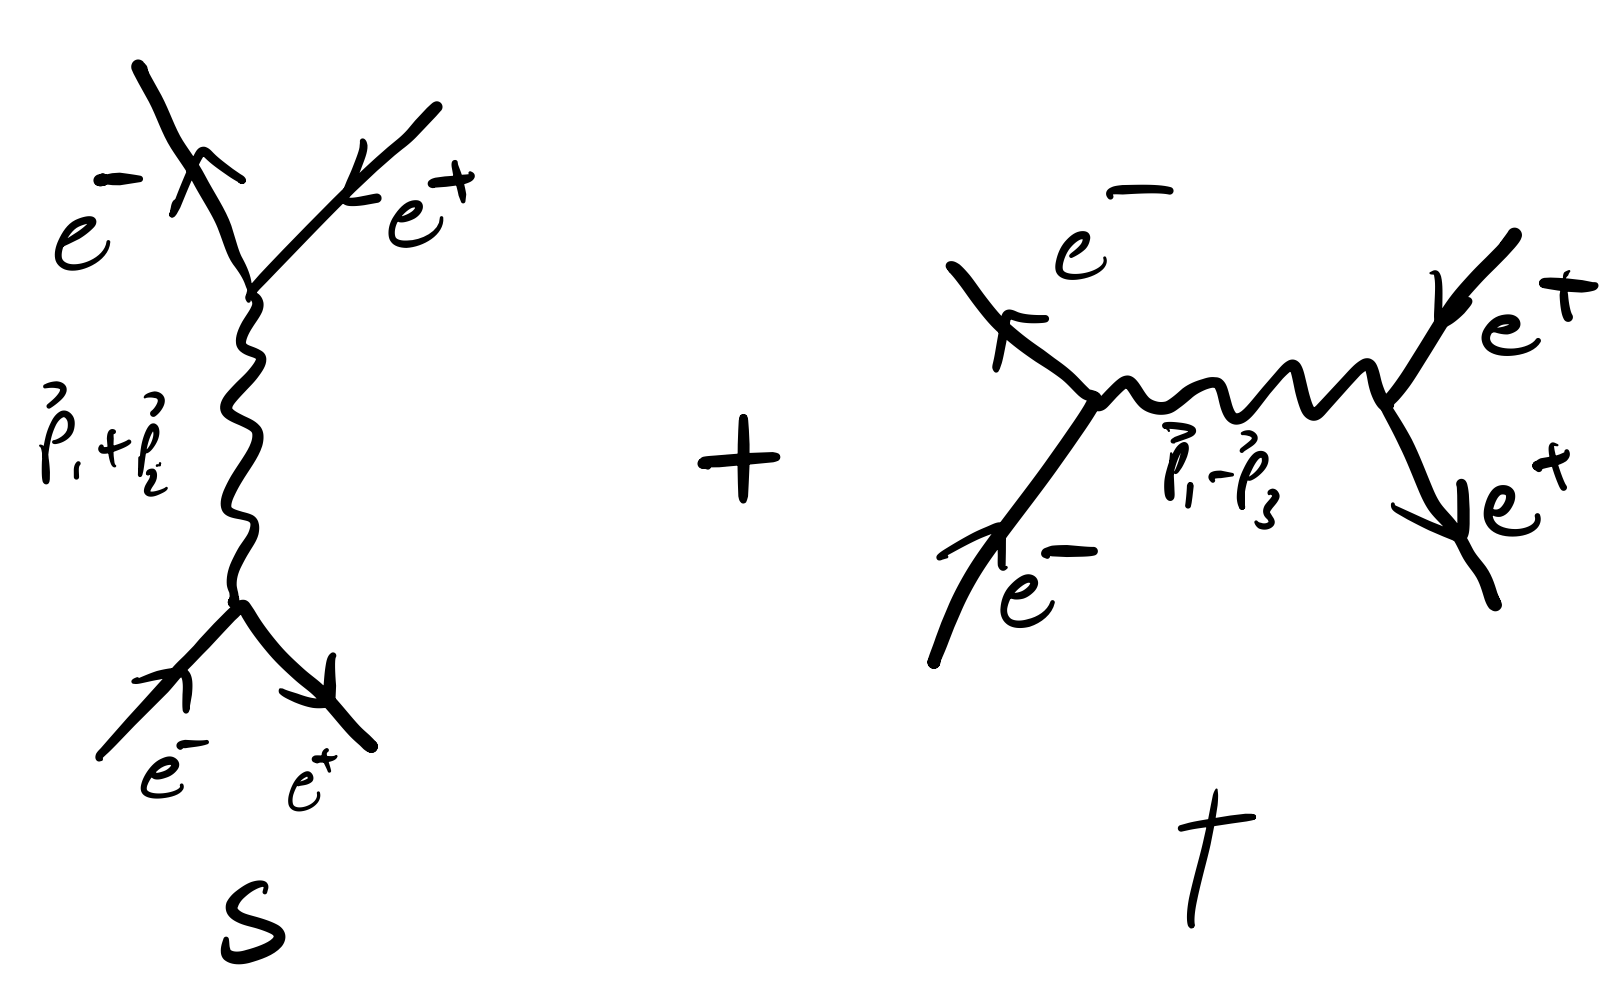
\includegraphics[scale=0.35]{Lectures/Images/lec13-stchannels.png}
\end{center}

The $u$-channel diagram below is not allowed as it has $\psi\psi A_\mu$:

\begin{center}
    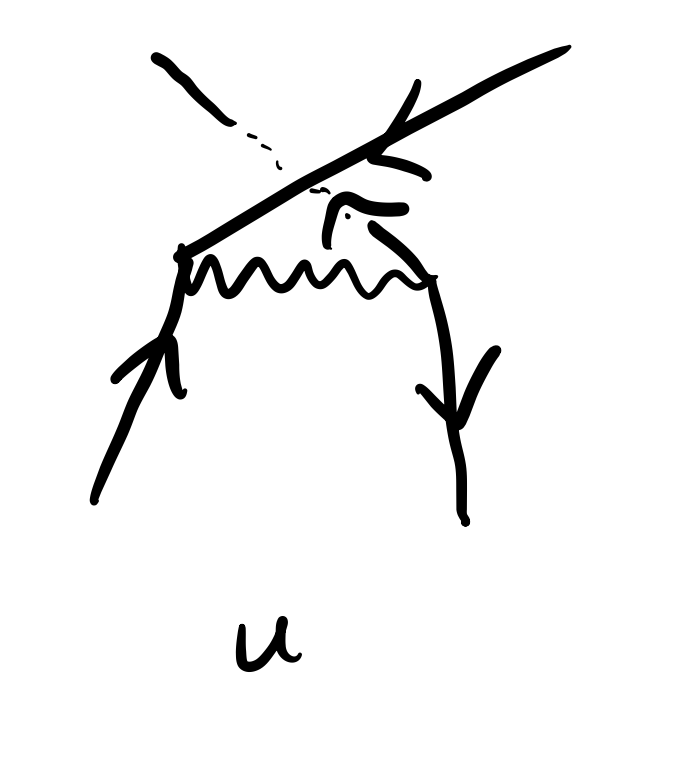
\includegraphics[scale=0.35]{Lectures/Images/lec13-uchannel.png}
\end{center}

So in summary we expect:
\begin{equation}
    \mathcal{M}_{e^-e^+ \to e^-e^+} = \frac{e^2}{s}(\bar{u}_3\gamma_\rho v_4)(\bar{v}_2\gamma^\rho u_1) + \frac{e^2}{t}(\bar{v}_2\gamma^\rho v_4)(\bar{u}_3\gamma_\rho u_1)
\end{equation}
and you check this on the homework.

\subsection{$e^+e^-\to\mu^-\mu^+$ - Summing over spins}
Going back to our result for the $e^+e^-\to\mu^-\mu^+$, if we know the momenta and all the spins, our result Eq. \eqref{eq:eemumu} is the final answer. A simpler answer arises if we sum over spins. This is also experimentally relevant if the spin of the particles is not measured.

The probability of an event is $\propto \abs{\mathcal{M}}^2$. Let's sum the probability for any outgoing set of spins:
\begin{equation}
    \abs{\mathcal{M}}^2 = \frac{e^4}{s^2}(\bar{u}_3\gamma^\rho v_4)(\bar{v}_4\gamma^\lambda u_3)(\bar{v}_2\gamma_\rho u_1)(\bar{u}_1\gamma_\lambda v_2)
\end{equation}
Let's sum over the outgoing states $s_3, s_4$ using the completeness relations:
\begin{equation}
    \sum_{s_3 = \pm}u_{s_3}(\v{p}_3)\bar{u}_{s_3}(\v{p}_3) = (-\slashed{p}_3 + M)
\end{equation}
\begin{equation}
    \sum_{s_4 = \pm}v_{s_4}(\v{p}_4)\bar{v}_{s_4}(\v{p}_4) = (\slashed{p}_4 + M)
\end{equation}
with $M = m_\mu$. We can now convert the sum over spins into taking the trace of a matrix:
\begin{equation}
    \sum_{s_3, s_4}\abs{\mathcal{M}}^2 = \frac{e^4}{s^2}\text{Tr}(\gamma^\rho(\slashed{p}_4 + M)\gamma^\lambda(\slashed{p}_3 - M))(\bar{v}_2\gamma_\rho u_1)(\bar{u}_1\gamma_\lambda v_2)
\end{equation}
Now we also average over all incoming spins $\frac{1}{4}\sum_{s_1, s_2}$:
\begin{equation}
    \frac{1}{4}\sum_{s}\abs{M}^2 = \frac{e^2}{s^2}\Tr(\gamma^\rho (\slashed{p}_4 + M)\gamma^\lambda(\slashed{p}_3 - M))\Tr(\gamma_\rho(\slashed{p}_1 - m)\gamma_\lambda(\slashed{p}_2 + m))
\end{equation}
with $m = m_e$. Now let's deal with the traces:
\begin{equation}
    \begin{split}
        \Tr(\gamma^\rho (\slashed{q} + M)\gamma^\lambda(\slashed{k} - M)) &= -m^2\Tr(\gamma^\rho\gamma^\lambda) + q_\alpha k_\beta\Tr(\gamma^\rho\gamma^\alpha\gamma^\lambda\gamma^\beta)
        \\ &= 4m^2\eta^{\rho\lambda} + 4(q^\rho k^\lambda + q^\lambda k^\rho - kq\eta^{\rho\lambda})
    \end{split}
\end{equation}
We have two traces, and the results are subsequently contracted, so:
\begin{equation}
    \begin{split}
        \frac{1}{4}\frac{1}{4}\Tr(\ldots) \Tr(\ldots) &= [M^2\eta^{\rho\lambda} + p_3^\lambda p_4^\rho + p_3^\rho p_4^\lambda - \eta^{\rho\lambda}p_3\cdot p_4][m^2\eta_{\rho\lambda} + (p^1_\rho p^2_\lambda + p^1_\lambda p^2_\rho + p^1 \cdot p^2 \eta_{\lambda\rho})]
        \\ &= 4m^2M^2 + M^2(-2)p_1 \cdot p_2 + m^2(-2)p_3 \cdot p_4 + 2(p_3 \cdot p_1) (p_2 \cdot p_4) + 2(p_3 \cdot p_2)(p_1 \cdot p_4) - 4(p_3 \cdot p_4)(p_1 \cdot p_2) + 4(p_3 \cdot p_4)(p_1 \cdot p_2)
        \\ &= 4mM^2 - 2(M^2p_{12} + m^2p_{34}) + 2(p_{13}p_{24} + p_{14}p_{23})
    \end{split}
\end{equation}
Thus the probability of scattering, ignoring spin, is proportional to:
\begin{equation}
    \frac{1}{4}\sum_{s_1s_2s_3s_4}\abs{\mathcal{M}}^2 = \frac{8e^2}{s^2}[2m^2M^2 - (M^2p_{12} + m^2p_{34}) + (p_{13}p_{24} + p_{14}p_{23})]
\end{equation}
Indeed this is independent of spin and only depends on Lorentz-invariant contractions of four-momenta $p_{ij} = p_i \cdot p_j$. Finally, let us convert to Mandelstam variables:
\begin{equation}
    s = -(p_1 + p_2)^2 = m^2 - 2p_{12} \stackrel{\text{p}-conservation}{=} -(p_3 + p_4)^2 = 2M^2 - 2p_{34}
\end{equation}
\begin{equation}
    t = -(p_1 - p_3)^2 = m^2 + M^2 + 2p_{13} \stackrel{\text{p}-conservation}{=} -(p_2 - p_4) = m^2 + M^2 + 2p_{24}
\end{equation}
\begin{equation}
    u = -(p_2 - p_4)^2 = m^2 + M^2 + 2p_{14} \stackrel{\text{p}-conservation}{=} -(p_1 - p_3)^2 = m^2 + M^2 + 2p_{13}
\end{equation}
Thus replacing the $p_{ij}$ in our probability expression:
\begin{equation}
    \boxed{\frac{1}{4}\sum_{s_1,s_2,s_3,s_4}\abs{\mathcal{M}}^2 = \frac{8e^2}{s^2}[t^2+ u^2 + 4s(m^2 + M^2) - 2(m^2 + M^2)^2]}
\end{equation}
Last quarter, we saw how to get a differential cross section out of this; as we obtained for scalars; at high-energies with $p \gg M,m$ this yields:
\begin{equation}
    \dod{\sigma}{\Omega} = \text{Const.}\cdot\frac{e^4}{E_{\text{CM}}^2}(1 + \cos^2\theta)
\end{equation}

\begin{center}
    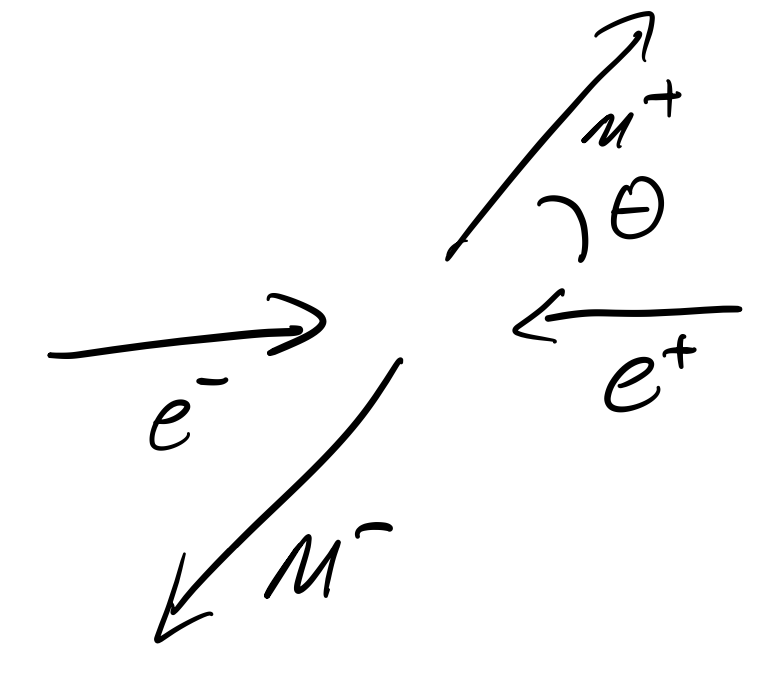
\includegraphics[scale=0.35]{Lectures/Images/lec13-angledependence.png}
\end{center}

See Schwartz (13.78) for details. What is the intuition for this expression? For scalars we found that $M = \lambda$ and $\dod{\sigma}{\Omega} = \frac{\lambda^2}{E_{CM}^2}$, coming from:

\begin{center}
    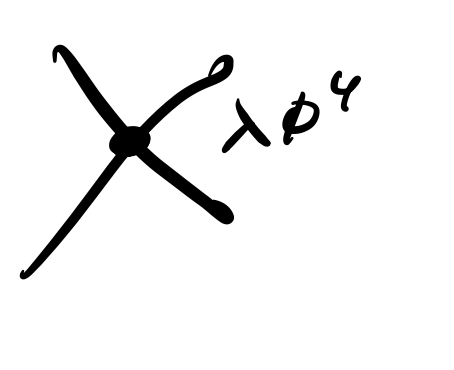
\includegraphics[scale=0.35]{Lectures/Images/lec13-scalarvertex.png}
\end{center}

Now, we have angle dependence. Why? It has to do with the spin. Because the electron/positron pair must create a photon to mediate their interaction, we need their helicities to align a helicity-1 photon state. If the helicities are all pointing out of the page/normal to the direction of propagation, we have exactly what we want. If instead they point in the plane of the collision, the helicities of muon no longer quite align and hence we get a $\propto (\cos\theta)^2$ dependence.

\begin{center}
    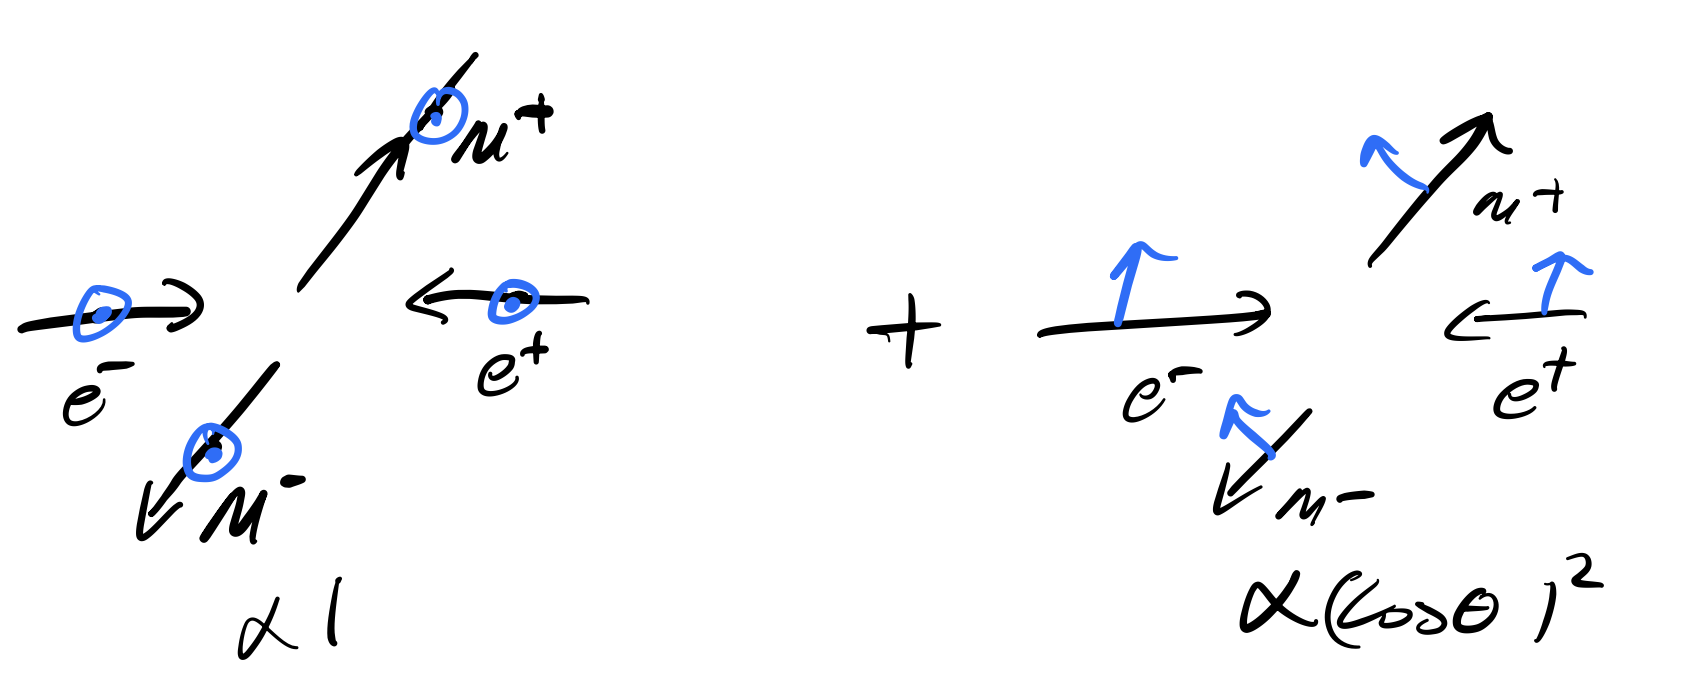
\includegraphics[scale=0.35]{Lectures/Images/lec13-twoparts.png}
\end{center}
